\section{问题描述与研究动机}
\subsection{场景、观测任务与固有挑战}
\label{sec:task}
图\ref{fig:scene}给出湖岸设施附近的目标应用场景。未知固定源位于物理允许的释放区域，气体在地形、障碍和局地风作用下传播。两架无人机组成同步测量单元，获取气体序列、采样位置与局地测风，并根据已有观测更新源位置判断和下一测量动作。背景图中的两机及轨迹用于说明测量任务，不是枫树岭S2的已验收浓度场。本文的单源任务与后续多机任务分配研究分开。

\begin{figure*}[t]
\centering
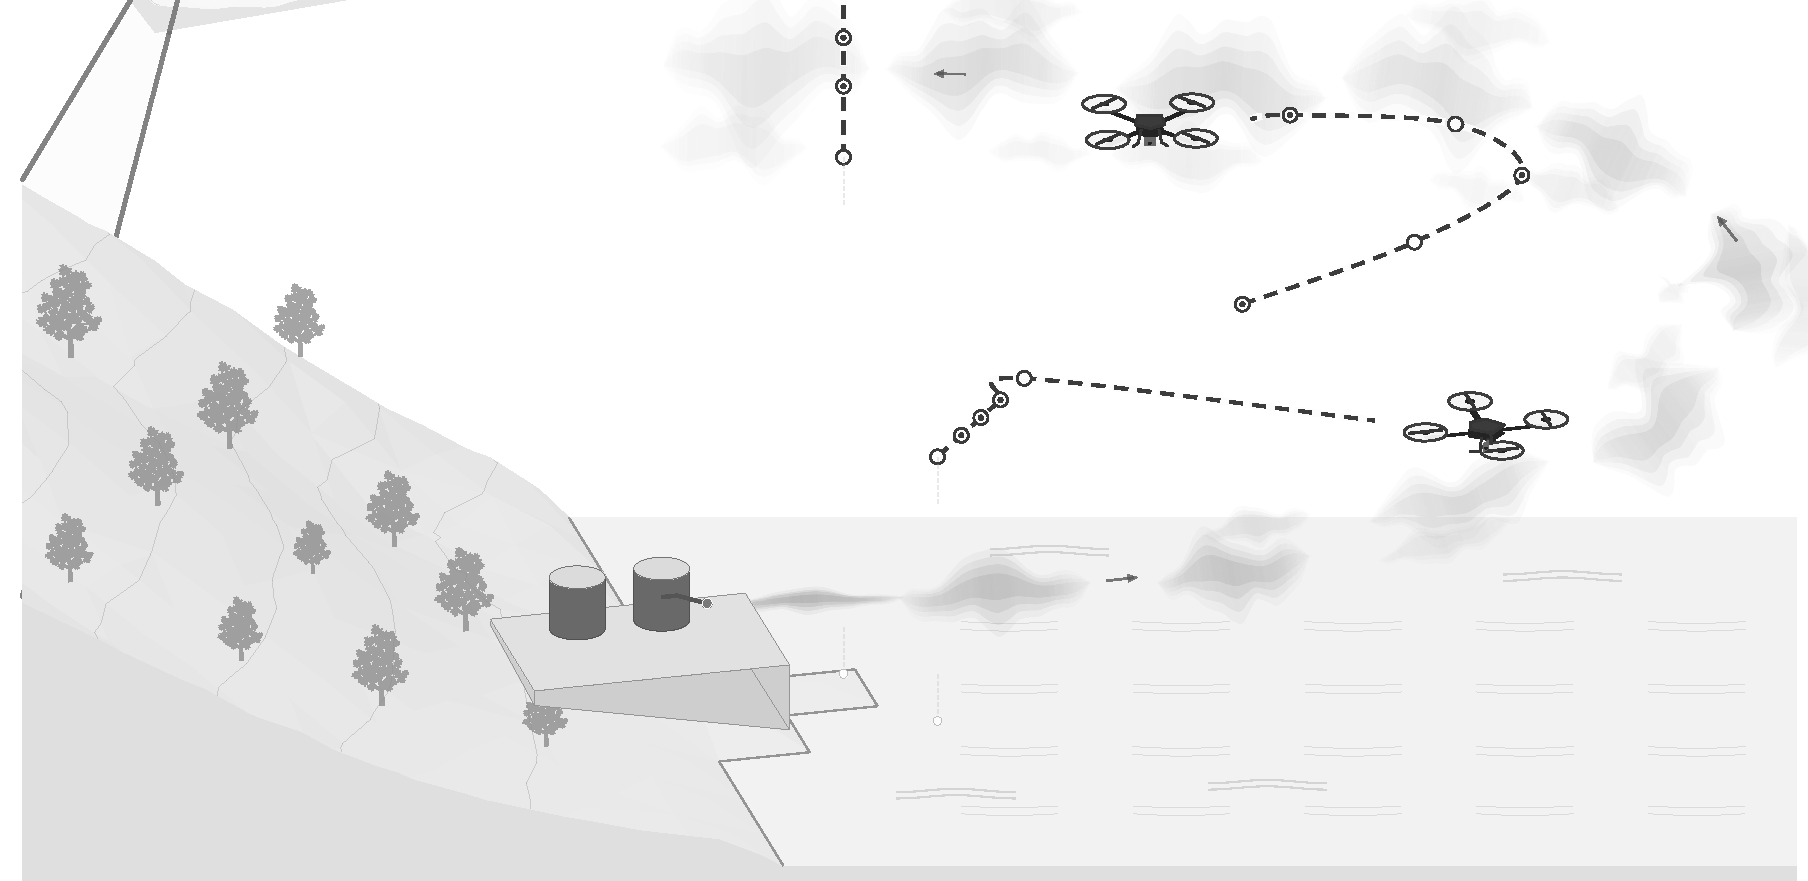
\includegraphics[width=0.97\textwidth]{figures/fig1_scene.pdf}
\caption{湖岸气体源定位目标应用场景。复用原可编辑研究背景图；双机同步测量的几何定义见图\ref{fig:geometry}。该图为概念示意，源概率图是本文主输出，未将场景图解释为已完成的湖陆风或三维羽流验证。}
\label{fig:scene}
\end{figure*}

记物理源可存在域为$\Omega_{\rm src}$，飞行可达域为$\Omega_{\rm fly}$，传感器有效采样域为$\Omega_{\rm obs}$。三者分别由释放条件、飞行安全及传感器安装位置确定，不能以二维导航自由格替代全部合法源。候选源集合为$\mathcal S=\{s_j\}_{j=1}^J\subset\Omega_{\rm src}$，$s_j=(x_j,y_j,z_j)^{\mathsf T}$，真实固定源为$s^*$。有限候选集合内的分类性能与连续未知源的定位精度分别评价。

以$t$表示决策或观测块编号，以$\tau_{t,n}$表示第$t$块中第$n$个样本的物理时间。左右传感器标记为$u\in\{L,R\}$，实际采样位置为$\mathbf x^u_{t,n}\in\R^3$，气体读数为$y^u_{t,n}$，局地测风为$\widehat{\mathbf v}^u_{t,n}$。原始同步观测块写为
\begin{equation}
 X_t=\big\{\tau_{t,n},\mathbf x^u_{t,n},y^u_{t,n},
 \widehat{\mathbf v}^u_{t,n}\big\}_{n=1,u\in\{L,R\}}^{N_t}.
 \label{eq:block}
\end{equation}
世界坐标、测点外参、两侧时钟及浓度单位需在形成$X_t$之前统一；不可用相邻世界、未来风或事后平移的真源历史拼成同步块。局地风仅在实际可用时进入算法，缺测和不具备竖直风分量必须保留标记。

给定源、传播状态及传感器参数，读数可统一表示为
\begin{equation}
 y^u_{t,n}=\mathcal G_{\psi_u}\!\left[
 C\!\left(\mathbf x^u(\tau),\tau;s_j,\eta\right),m^-_{u,t}
 \right](\tau_{t,n})+\varepsilon^u_{t,n}.
 \label{eq:sensor}
\end{equation}
其中$C$为三维物理浓度，$\eta$包括未知释放强度、传播条件等干扰量，$\mathcal G_{\psi_u}$表示经校准的传感器动态，$m^-_{u,t}$为该块开始前的实际响应状态，$\varepsilon^u_{t,n}$为测量噪声。原生GADEN及GADEN-RT为候选传播和受体浓度提供仿真工具\ccite{Monroy2017GADEN,Ojeda2025GadenRT}，但仿真浓度与真实PID读数不能不经说明地等同。第5节的归档实验使用理想零延迟浓度查询，不检验式\eqref{eq:sensor}中的真实传感器动态。

地图和障碍为$G$，冻结训练资料及事前配置为$\mathcal D_{\rm tr}$。本稿以$X_t$表示用于M1的同步采样窗；截至第$t$步结束已经取得的行进期气体、位置、运动方向及可用局地风另记为$H_t^{\rm tr}$。完整已发生历史定义为$\mathcal F_t=\sigma(G,\mathcal D_{\rm tr},X_{1:t},H_t^{\rm tr},a_{1:t})$，因此行进期数据虽不进入当前驻留块似然，也属于策略实际可见的信息。动作$a_t$包含两机实际路径、测量中心、基线长度与方向、采样高度及驻留时间，基于$\mathcal F_{t-1}$及与环境独立的控制随机数选定，并在新观测出现前固定。任务资源由移动、停留、传感器数量和计算成本共同约束。定位主输出为源质量$\pi_t(s_j)$及其二维投影
\begin{equation}
 P_t(g)=\sum_{j:\Pi(s_j)\in g}\pi_t(s_j),\qquad
 \sum_g P_t(g)=1,
 \label{eq:projection}
\end{equation}
其中$\Pi(s_j)=(x_j,y_j)$，$g$为二维源图单元。候选源高度未知时应将合法高度作为候选或共享机制建模，再按式\eqref{eq:projection}边缘化；不能删除不在导航平面的源后仍声称覆盖其物理位置。输出同时保留MAP集合、概率覆盖情况及当前审计列表，后者不等同于概率图。

这一任务具有三方面固有困难。其一，间歇传播与未知风历史使相同源的有限窗响应变化，不同源也可能产生近似观测。其二，有限测点与有限带宽限制可观测尺度，两侧延迟不一致甚至可产生并不存在的运动线索。其三，飞行几何、源位置支持和受体体积处于不同尺度，空间合法性不能由单一地图替代。这些困难独立于所采用的定位算法；高保真三维预测、额外测量平台或更长历史是否有用，最终都需由源判别结果说明。

\subsection{原生PMFS计算链及具体研究动机}
\label{sec:motivation}
PMFS利用局地浓度与风构造空间气体命中概率和采样置信度，通过候选源的简化二维丝团传播预测命中图，再按地图兼容程度得到源位置分布。其主动选点利用源分布加权的候选响应方差与未观测置信度\ccite{Ojeda2024PMFS}。图\ref{fig:pmfs}复用V7中对原方法的可编辑示意。这里将论文原理与具体代码版本分开：实现审计固定于作者仓库提交\texttt{4e141e1}，项目O24的作者代码来源固定于\texttt{a8d5a76}，未将前一版本的实现细节当作后一版本的实跑结论\ccite{V7Archive}。

\begin{figure*}[t]
\centering
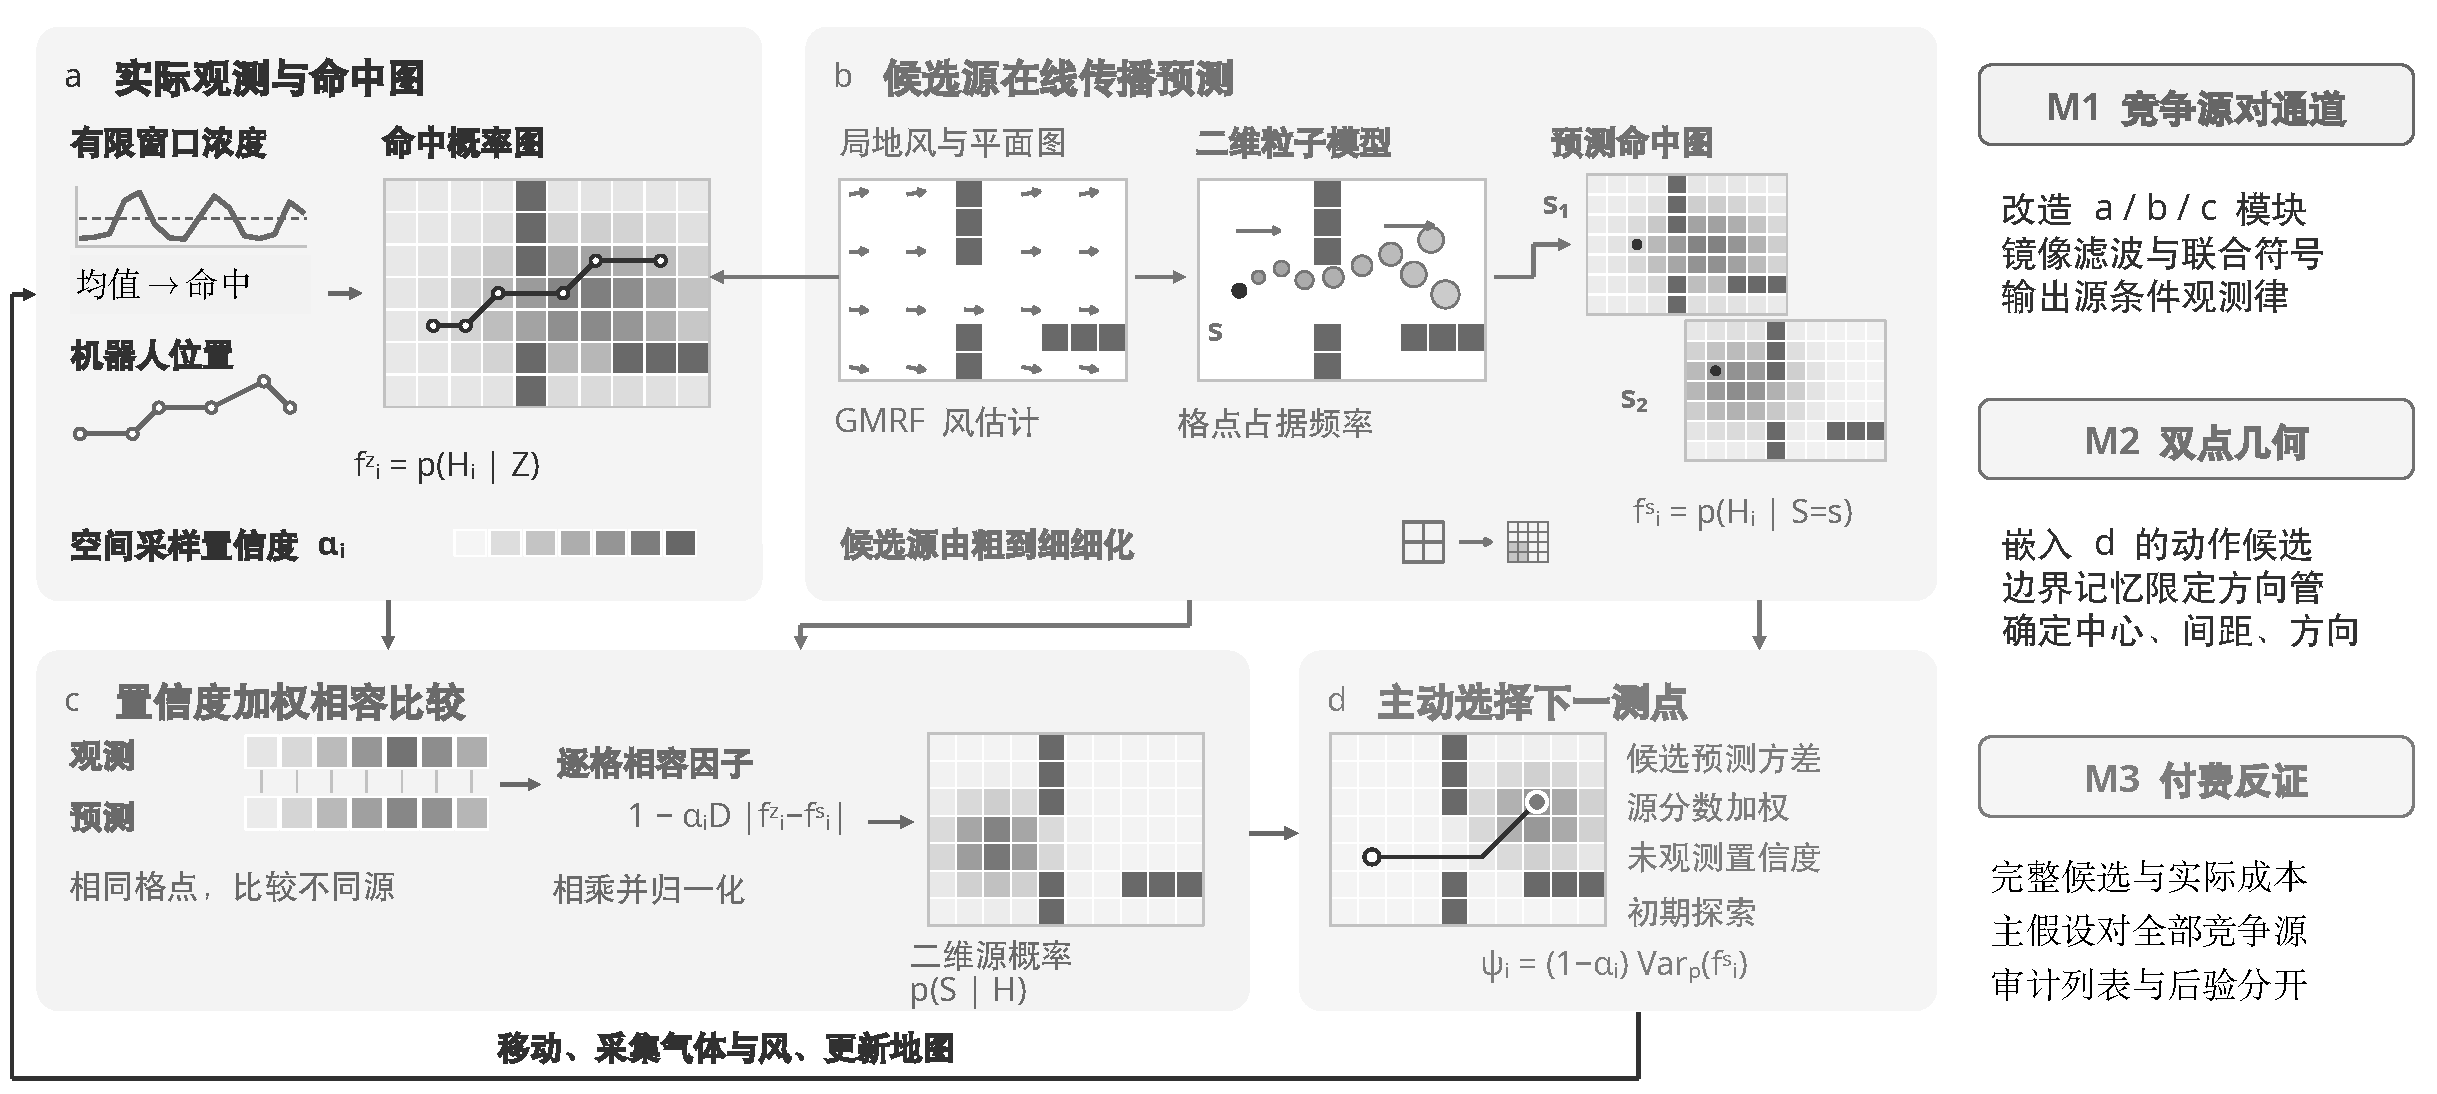
\includegraphics[width=0.98\textwidth]{figures/fig2_pmfs.pdf}
\caption{原生PMFS的观测命中图、候选传播、兼容评分和主动选点，以及本文对应的观测表示与决策接口。图源为V7可编辑方法图第1页；正文区分论文原理和固定代码版本。二维命中图与二维源概率图具有不同含义。}
\label{fig:pmfs}
\end{figure*}

上述被审计实现对有限停留窗内的平均浓度阈值化，再以风相关空间核传播命中事件并累积地图信息。令$p_{i,t}$为第$i$格当前观测命中概率，$h_{i,t}(s_j)$为候选预测频率，$c_{i,t}$为采样置信度，$D$为固定兼容系数，则源评分的实际结构为
\begin{equation}
 \widetilde\pi^{\rm PMFS}_t(s_j)=
 \prod_{i\in\mathcal V_{\rm free}}
 \bigl[1-c_{i,t}D\lvert p_{i,t}-h_{i,t}(s_j)\rvert\bigr].
 \label{eq:pmfscompat}
\end{equation}
归一化后的评分覆写源图，历史主要通过累计命中图进入。式\eqref{eq:pmfscompat}不额外乘前次源后验，因此不能将其错误描述成每轮重复乘入旧后验。相同局地事件可影响多个地图单元，这些单元间的依赖及观测/预测读出定义是否匹配，才是需要控制实验检验的问题。该版本实际选点所用的主要代理量为
\begin{equation}
 V_t(x)=\bigl[1-c_t(x)\bigr]
 \operatorname{Var}_{\pi^{\rm PMFS}_t}
 \{h_t(x;S)\}.
 \label{eq:pmfsplanning}
\end{equation}
它体现候选预测分歧，但不是已校准的有限驻留传感器互信息。测量噪声、带宽和候选分布形状均可能改变实际可分性，不能仅凭均值方差较大推断单位时间的源信息较多。

表\ref{tab:motivation}将研究动机限定在已有证据能够支持的层次。B4错误高置信是停止条件与真实位置准确性不一致的实例；M4/RK对照说明预测损失与定位目标不等价；有限观测相容性记录说明少量观测可能不足以排除多个源。各例的数据权限、源支持、观测窗口和模型不同，不能合并成一个已经确认的物理根因。

\begin{table*}[t]
\centering\small
\caption{动机证据、允许推论及其限制。历史诊断与V7开发对照不是同一数据集上的方法排名。}
\label{tab:motivation}
\begin{tabularx}{\textwidth}{p{1.4cm}Y Y Y}
\toprule
记录 & 已发生事实 & 支持的研究问题 & 不能推出的结论\\
\midrule
B4 & 官方运行成功标记为真，源图方差约0.329，Top-5\%位置误差5.112\,m；锁定错/真代表源兼容分数比约14874.6\ccite{EvidenceB4} & 源图集中和停止标记应与位置准确性、覆盖率分别检验 & 尚未唯一识别风、观测算子、源高度或相关评分为根因\\
M4 / RK & M4场MSE改善而强对照与新表示均4/4判对；RK2-L相对S的连续MSE下降约29.22\%，源NLL约1.22\%，Top-1均4/4\ccite{EvidenceRK} & 优化目标需落到候选源排序与概率质量 & 浓度预测改善不能自动证明定位增益，复合分数不等于校准后验\\
有限观测相容性 & 既有R3相关汇总报告少量观测下多个候选仍相容；其窗口级原收据尚未完全恢复\ccite{V7Archive} & 应检验给定动作下竞争源是否实际可分 & 本稿不把汇总数当新复核实验，也不把容错能力当源可辨识保证\\
V7原生开发 & 4个DEV世界普通单点与完整双点均4/4；M1为2/4，动态镜像通道选择数为0\ccite{V7Native} & 表示压缩与训练选择目标可能未保留已有判别信息 & 不能归因于PMFS，也未否定所有镜像嗅觉结构\\
\bottomrule
\end{tabularx}
\end{table*}

具体而言，静态命中率未必充分表达双点关系：左右两侧边缘命中率相同的两个过程，可以分别呈现同步与交替检出；其联合分布可能不同。只有这种差异在实际传感器读出后仍稳定关联源身份，才构成定位信息。反之，在简单匀速传播中，两测点到达时差可能主要由基线和风速决定，不能自动换算为源距离。M1据此采用源条件联合标定，而不把方向判断直接称为源定位。

错误后验还可能影响采样：若动作只按高后验源加权，低后验真源对应的辨识位置可能长期得不到访问。这是可分析的决策风险，并非B4已被证实的唯一失败链。M2改变可取得的原始观测几何，M3保留对完整源集的付费挑战，两者的作用分别由测量几何和恢复消融检验。增加双机资源带来的收益须与相同资源下的普通联合模型分开。

\subsection{科学问题与总体方案}
本文研究的问题是：\textbf{在有限飞行、驻留和标定样本预算下，如何将双侧观测中的源相关差异转化为可靠证据，并主动取得能够反驳竞争源的新测量，持续输出二维源概率图？}核心研究对象是源条件观测律$p_t(X_t\mid s_j,r,a_t,\mathcal F_{t-1})$，其中$r$表示在一个比较阶段共享的有限干扰机制。当前有限通道标定的是冻结编码$Z_t=\phi_{a_t}(X_t)$在该观测律下形成的推前分布$p_t^Z(z\mid s_j,r,a_t,\mathcal F_{t-1})$，而非原始高维$X_t$的分布本身；它对编码观测律的估计精度和跨源泛化能力需要单独验证。后文条件性理论要求观测律针对上述完整历史成立；把行进期信息写入$\mathcal F_t$只是澄清理论前提，不表示当前固定条件表已实现对该信息的全部条件化。

\begin{figure*}[t]
\centering
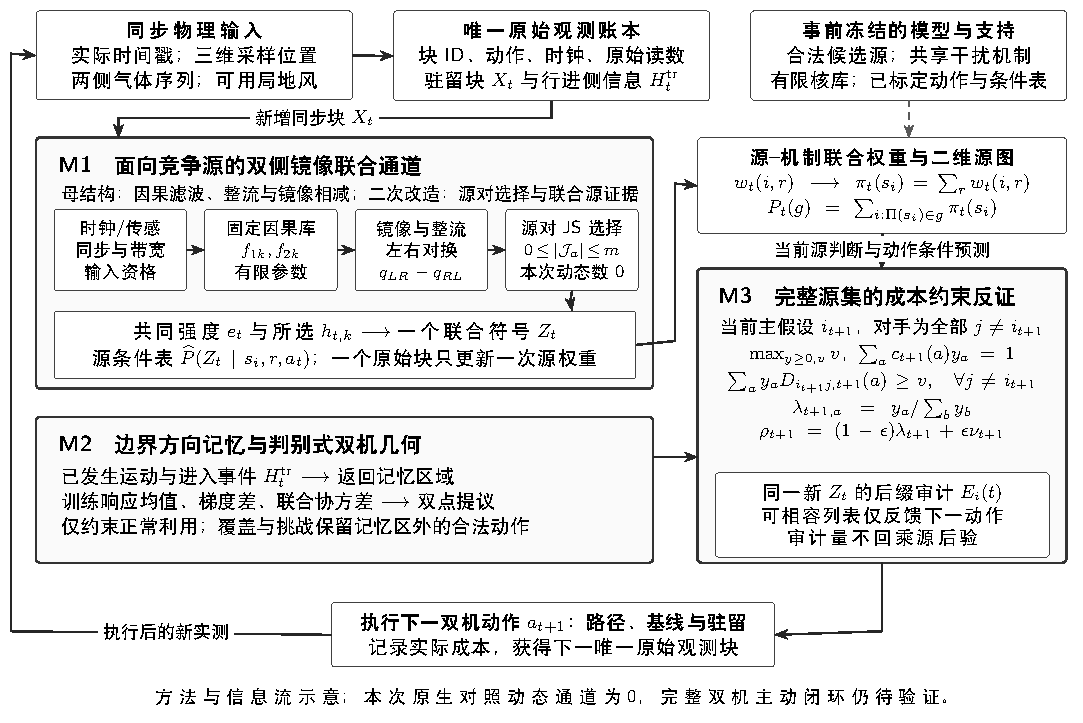
\includegraphics[width=0.98\textwidth]{figures/fig3_v7_framework.pdf}
\caption{三个模块的统一信息关系。完成第$t$块观测后规划第$t+1$步动作。依据V7可编辑方法图第2页重绘并修订，统一共享干扰机制$r$及主假设对完整竞争源的成本分配。M1产生联合观测符号，M2提出判别几何，M3选择有成本的反证动作；新观测后缀审计不回乘源后验。图示为方法设计，不表示完整原生闭环性能已验证。}
\label{fig:framework}
\end{figure*}

图\ref{fig:framework}中，M1将同步块转换为共模与镜像响应的联合符号$Z_t$，更新源--机制联合权重并边缘化输出$P_t(g)$；M2利用已发生的边界事件、运动方向及训练源响应形成合法双机动作；M3比较完整源集上的动作条件差异，计入实际成本，并以新后缀检查当前源解释。原始观测、几何记忆、源后验和审计量各有不同含义，不能互作独立气体证据重复计数。

设$Z_t=\phi(X_t)$为固定后或以过去信息选定的确定性编码，由数据处理不等式\ccite{Cover2006}
\begin{equation}
 I(S;Z_t\mid a_t,\mathcal F_{t-1})
 \le I(S;X_t\mid a_t,\mathcal F_{t-1}).
 \label{eq:dpi}
\end{equation}
因此M1不会创造原始观测中不存在的源信息。其待检验价值是在有限样本与有限模型容量下保留可泛化的判别结构，或者降低同等判别质量所需的标定与计算成本。M2通过实际改变测量位置和双机基线，才可能改变可获得的原始信息；M3控制这些动作的分配及已有判断的复核。三模块的设计完整性、条件性数学成立和实际性能验证分别报告，不以其中一项替代另外两项。
